\chapter{Introduction}
With this project, we have studied, analyzed and provided a prototype solution that models the business processes of \textbf{Caseificio Mambelli} so
that they can benefit from strong technological and digital support going in a direction of integration, resource-saving and innovation.

Following the domain analysis conducted with domain experts, which areas could benefit from Digital Twin support were identified.
As a project challenge, Digital Twin modeling was conducted following some of the Domain Driven Design methodologies.

One of the issues that domain experts have raised is that the information and reports that the machines generate are difficult to find.
Each manufacturer makes its reports or data available through very different formats and applications; all of which make it very difficult
and inconvenient to extrapolate this data and cross-reference it to gain insight into the effectiveness of business processes.
Therefore, through Digital Twin, we want to significantly improve this issue by going in a direction of uniformity of access to machinery
information.
Another aspect that we want to improve is to integrate machinery more closely with the corporate factory system so that they operate in unison.
Finally, we have envisioned how Digital Twins can make machinery smarter by, for example, predicting its breakdowns and preventing failures while
minimizing outages.

All proposed analyses and solutions were made possible through feedback and support from domain experts.
The added value to this project from our point of view is dictated by the fact that it was possible to interact with them and collaborate to find
solutions to concrete problems.

In the intervening period for the development of the project, the company has made adjustments for ``Industria 4.0'' giving us the opportunity to
analyze what requirements are required and what possible improvements can be applied to move in a direction of innovation.

In the following sections, we will describe the current problems the company is facing and the possible solutions that we have proposed.

\section{Interoperability}
The problem of interoperability in the industrial context has been evident for years now~\cite{LIAO201712434}: each manufacturer produces closed systems, and interoperability with other machines succeeds only if the two parties agree on how to exchange data.
Collaborations between companies often result in tensions and disagreements slowing system development and generating a sub-optimal quality product.
In addition, such collaborations are created ad-hoc, so the methodologies and tools used can vary significantly going to making further integration
with other systems or devices difficult if not impossible.

In the manufacturing domain, interoperability represents a characteristic of a manufacturing system in which its components are capable of exchanging information with one another, using the information that has been exchanged.
Studies have been conducted on how interoperability is viewed at the industrial level. One study found that the automotive industry is strongly interested in achieving a high degree of interoperability, whereas the food industry perceives almost no need to have interoperable systems between them~\cite{LIAO201712434}. Only the 16\% of the food industry is interested in achieving a high degree of interoperability, compared with the 60\% of the automotive industry (Figure~\ref{fig:interoperability}).

\begin{figure}[h]
	\centering
	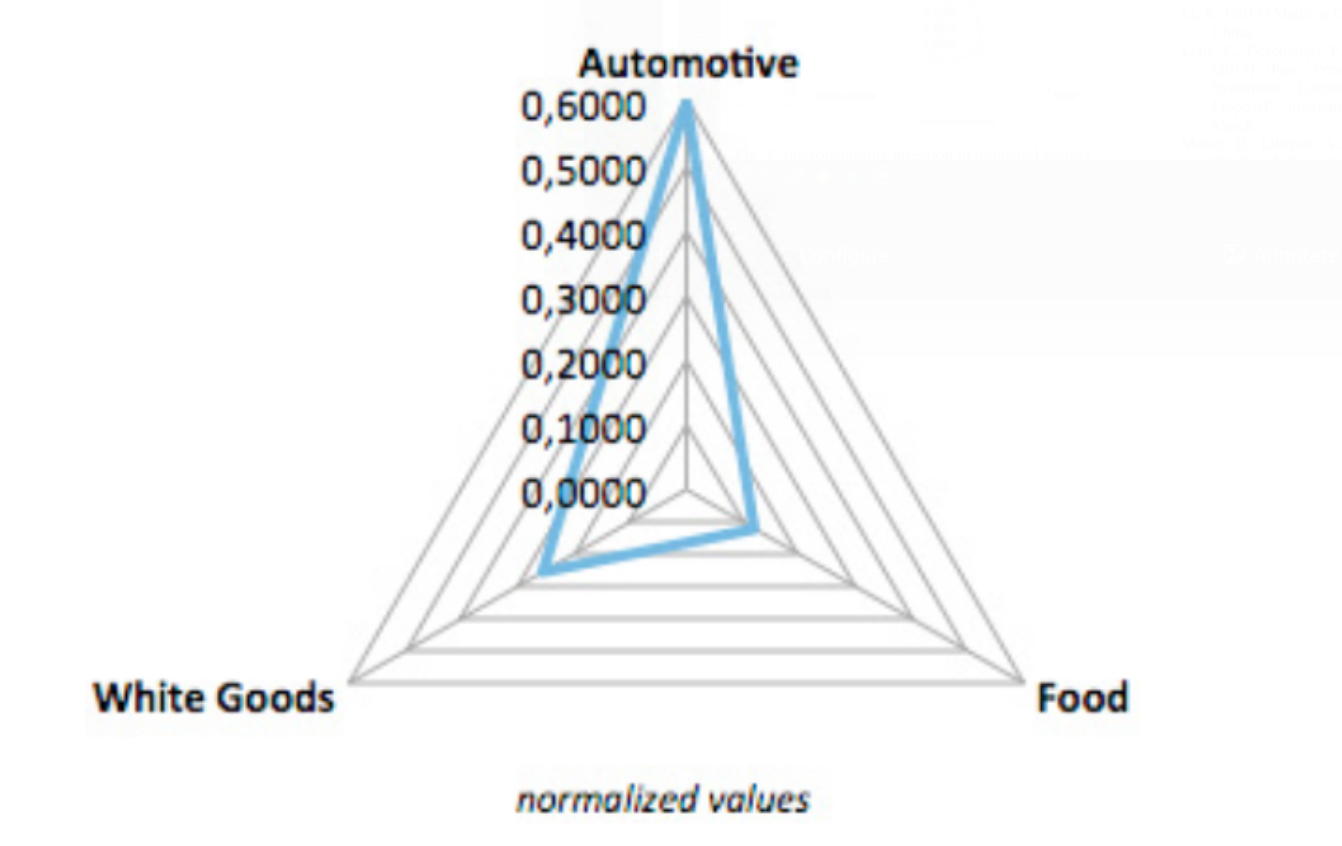
\includegraphics[width=0.6\textwidth]{img/interoperability.png}
	\caption{Interoperability attention in industrial sectors}
	\label{fig:interoperability}
\end{figure}

The results provided by the study are corroborated by the fact that domain experts initially did not perceive interoperability as beneficial, but
with the advent of \textit{Industry 4.0}, they have realized how interoperability is critical to the proper functioning of the system.

Currently, aspects of interoperability between machines are not present in the company.
Each machine in the production and packaging line is manually configured by an operator.
As can be easily guessed, this kind of operation can be error-prone, so having interoperability between machines that enable the communication of
information needed for that specific processing turns out to be a fundamental requirement in \textit{Industry 4.0}

Over time, several frameworks and standards have been proposed that aim to achieve a high degree of interoperability in the Industrial Internat of
Things. Among the most promising and interesting is the W3C Web of Things specification.
This specification keeps the promise to counter the fragmentation of the Internet of Things by defining a Web-based abstraction layer for existing
platforms, devices, gateways and services.
By complementing existing standards, it enhances interoperability thereby reducing the risk for investors and customers.
This will also enable the rapid growth of open markets for devices and services.

\begin{figure}[h]
	\centering
	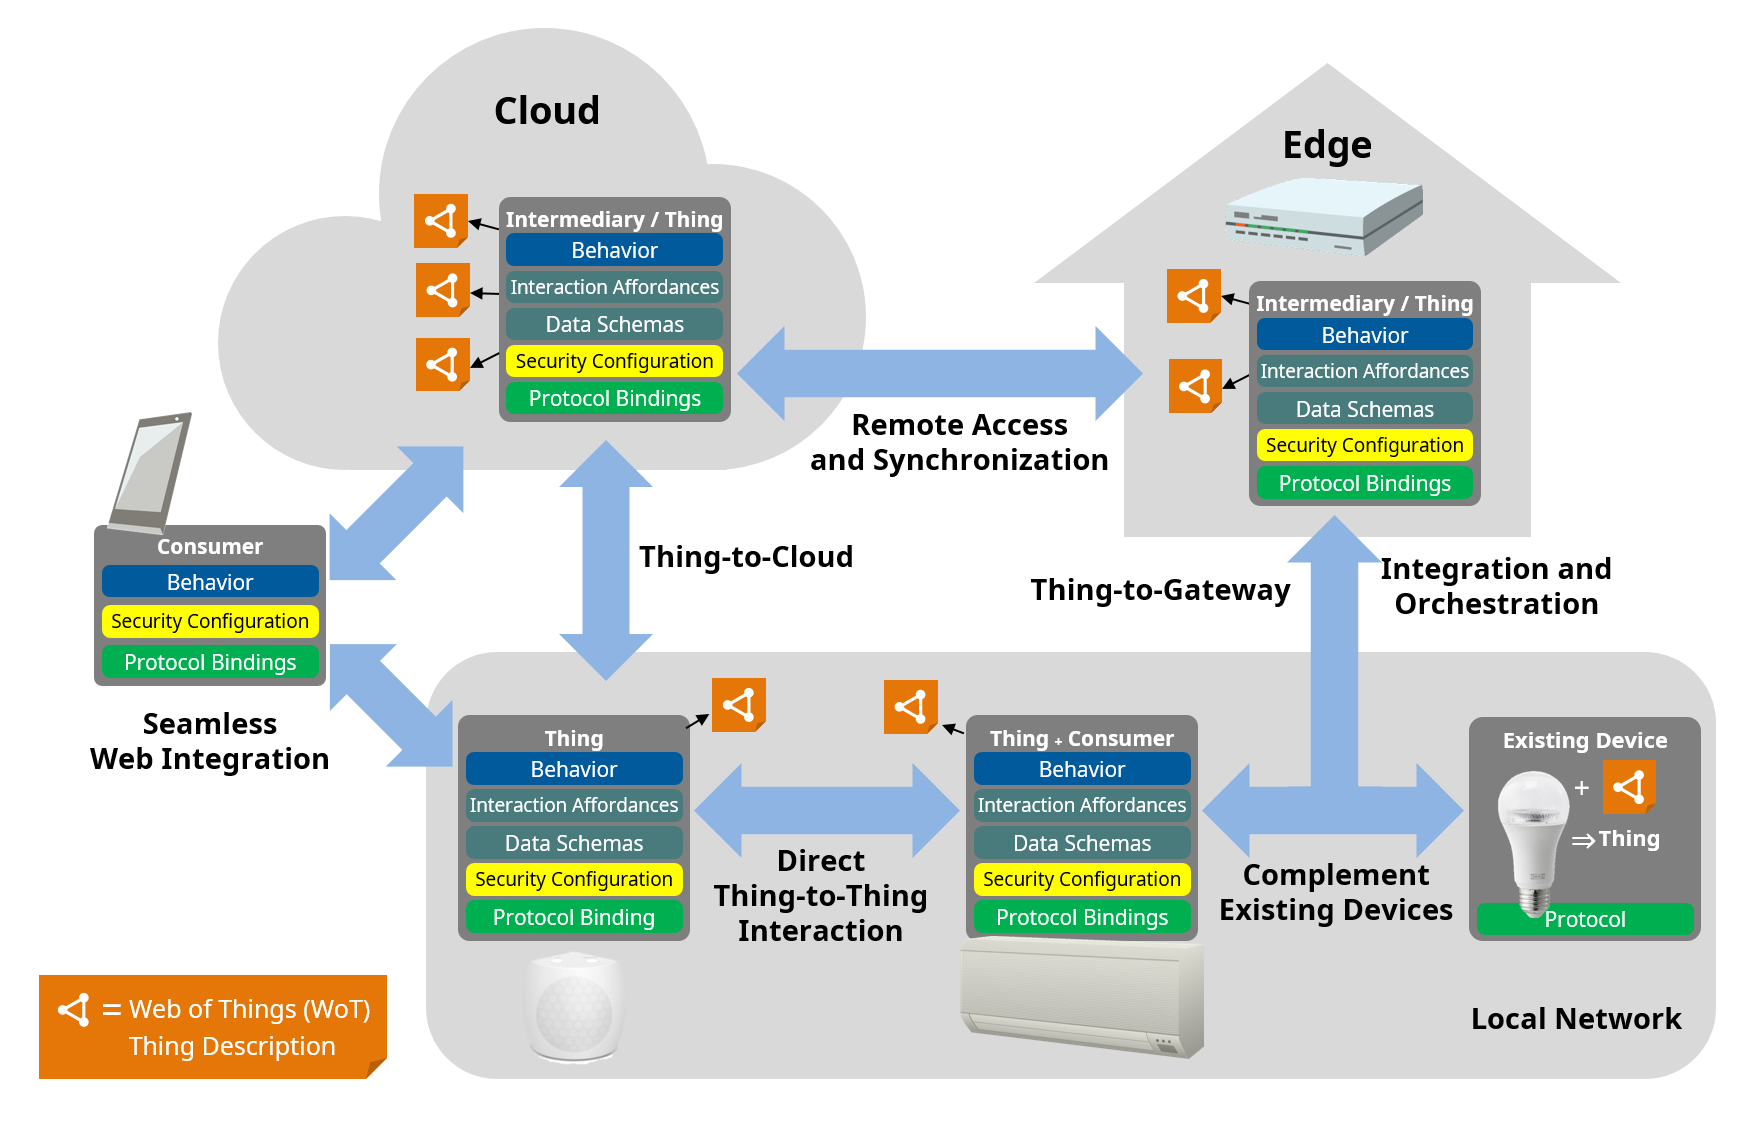
\includegraphics[width=0.7\textwidth]{img/wot.png}
	\caption{Web of Things architecture}
	\label{fig:iot}
\end{figure}

The Web of Things architecture (Figure~\ref{fig:iot}) shows how the interoperation between devices and systems is the main aspect.
In our opinion, the WoT specification is one of the most promising and interesting specifications for the development of interoperable systems.
Moreover, this specification joint with the Digital Twin pattern could represent a fundamental step towards interconnected digital systems.

\section{Industria 4.0}
